\section{Analisi dei Requisiti}
\labelsec{ReqAnalysis}
%===========================================================================
\subsection{Casi D'Uso}
\labelssec{UseCases}

\begin{figure}[ht]
\centering
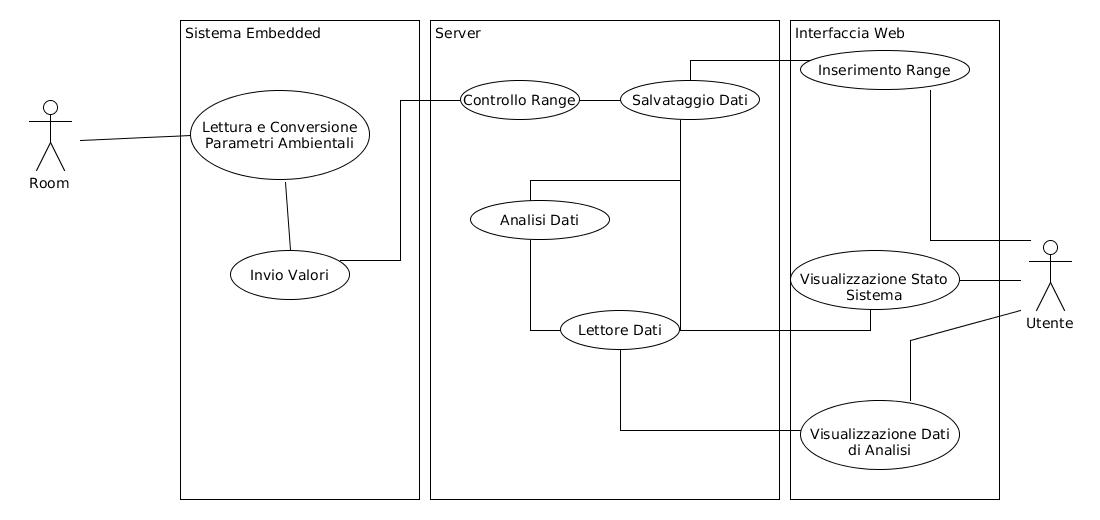
\includegraphics[width=\textwidth]{Figures/UseCases.jpg}
\caption{Casi d'Uso}
\end{figure}

Nell'immagine sopra si possono vedere quali sono le macro operazioni principali effettuate dal sistema e le interazioni con l'esterno. In particolare gli attori che interagiscono con il sistema saranno:

\begin{itemize}
  \item La stanza: con questo attore si intendono i vari parametri che si possono rilevare attraverso i sensori e che quindi saranno di input per il sistema.
  \item Utente: con questo attore rappresenta l'utente che puo' interagire con il sistema.
\end{itemize}

Il sistema \'e stato volutamente suddiviso in tre parti distinte con l'idea di seguire un modello MVC dove per\'o la parte di modello non viene aggiornato attraverso l'input inserito dall'utente, ma direttamente dall'input dei sensori. L'organizzazione hardware ha fortemente influito su questa suddivisione.

\'E inoltre possibile visualizzare le macro operazioni che devono essere effettuate e modellate dal sistema. Si vedano gli scenari di seguito per avere una piu' dettagliata visualizzazione dell'interazione tra le varie parti che lo schema sovrastante vuole rappresentare.


\subsection{Scenario}
\labelssec{Scenarios}

In questa sezione verranno illustrati le principali modalita' di utilizzo del sistema, includendo anche varianti che esulano da quello standard. Tutti gli scenari elencati di seguito riguardano l'utente e di conseguenza si prevede l'accesso da parte di questo all'interfaccia di input.

\subsubsection{Inserimento Range}

\begin{enumerate}
  \item Attraverso un apposito men\'u l'utente \'e in grado di accedere alla funzionalit\'a di settaggio dei range associati ai parametri ambientali.
  \item Il server sa gia' i sensori che sono collegati al raspberry, per via di un protocollo di comunicazione allo startup del sistema, e quindi l'utente e' in grado di visualizzare i controlli relativi ad ogni tipologia di sensore attualmente connesso. Conseguentemente l'utente e' in grado di modificare tali intervalli.
  \item Al termine della modifica degli intervalli l'utente dovr\'a confermare le modifiche attraverso un'apposito pulsante.
  \item Il sistema mostra un messaggio di conferma o di errore.
\end{enumerate}

\subsubsection{Visualizzazione Stato Realtime}

\paragraph{} All'accesso del sistema l'utente visualizza lo stato realtime dei valori dei sensori ed eventuali notifiche:
\begin{itemize}
  \item Se i valori vanno oltre gli intervalli correnti.
  \item Sullo stato dei sensori (malfunzionamenti - disconnessioni)
\end{itemize}

In questa modalita' l'utente non puo' effettuare alcuna operazione.

\subsubsection{Visualizzazione Dati}

\paragraph{} Attraverso un apposito men\'u l'utente \'e in grado di accedere alla visualizzazione dei dati storici dei vari sensori.

\subsection{Modello del Dominio}

\subsection{Piani di Test}

